
\usetikzlibrary{shapes.geometric}
\tikzset{
dot/.style = {circle, fill, minimum size=#1,
              inner sep=0pt, outer sep=0pt},
dot/.default = 6pt % size of the circle diameter 
}
 \renewcommand{\familydefault}{\sfdefault}

%\begin{document}
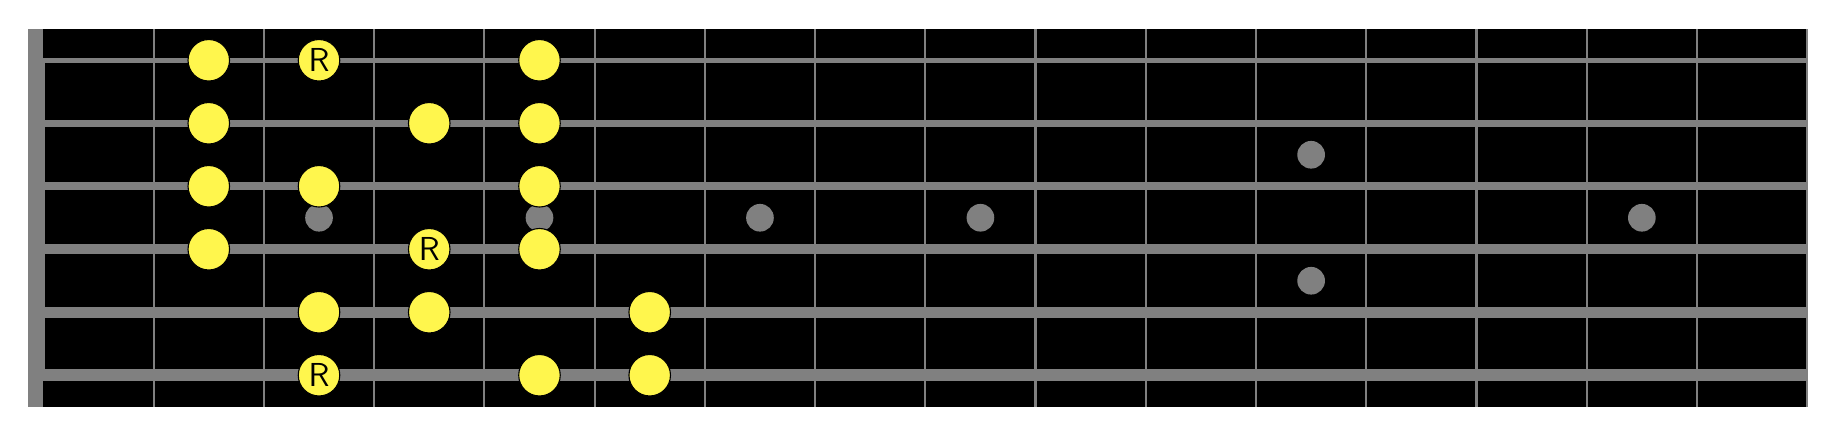
\begin{tikzpicture}[scale=1]
	\def \h{0.8}
	\def \fret{1.4} % 1.6
	\def \L{ 16*\fret }
	\def \dot_size{5pt}
	\def \circ_size{15pt}
	
	\fill[black, line width=2] (0.0,-0.4) rectangle (16*\fret,4.4);
	\fill[black!50!white, line width=2] (-0.2,-0.4) rectangle (0,4.4);
	
	% Strings
	\draw[color=black!50!white, line width=2.0]  (-0.1, 5*\h) -- (\L,5*\h); % E
	\draw[color=black!50!white, line width=2.5]  (-0.1, 4*\h) -- (\L,4*\h); % B
	\draw[color=black!50!white, line width=3.0]  (-0.1, 3*\h) -- (\L,3*\h); % G
	\draw[color=black!50!white, line width=3.5]  (-0.1, 2*\h) -- (\L,2*\h); % D
	\draw[color=black!50!white, line width=4.0]  (-0.1, 1*\h) -- (\L,1*\h); % A
	\draw[color=black!50!white, line width=4.5]  (-0.1, 0*\h) -- (\L,0*\h); % E
	
	% Frets 0
	\draw[color=black!50!white, thick]  (-0.1, 0) -- (-0.1,5*\h); 
	\draw[color=black!50!white, thick]  (0, 0)   -- (0,5*\h); 
	
	% Fret 1-15
	\draw[color=black!50!white, thick]  (\fret,   -0.4)   -- (\fret,4.4);   
	\draw[color=black!50!white, thick]  (2*\fret, -0.4) -- (2*\fret,4.4); 
	\draw[color=black!50!white, thick]  (3*\fret, -0.4) -- (3*\fret,4.4); 
	\draw[color=black!50!white, thick]  (4*\fret, -0.4) -- (4*\fret,4.4); 
	\draw[color=black!50!white, thick]  (5*\fret, -0.4) -- (5*\fret,4.4); 
	\draw[color=black!50!white, thick]  (6*\fret, -0.4) -- (6*\fret,4.4); 
	\draw[color=black!50!white, thick]  (7*\fret, -0.4) -- (7*\fret,4.4); 
	\draw[color=black!50!white, thick]  (8*\fret, -0.4) -- (8*\fret,4.4); 
	\draw[color=black!50!white, thick]  (9*\fret, -0.4) -- (9*\fret,4.4); 
	\draw[color=black!50!white, thick]  (10*\fret, -0.4) -- (10*\fret,4.4); 
	\draw[color=black!50!white, thick]  (11*\fret, -0.4) -- (11*\fret,4.4); 
	\draw[color=black!50!white, thick]  (12*\fret, -0.4) -- (12*\fret,4.4); 
	\draw[color=black!50!white, thick]  (13*\fret, -0.4) -- (13*\fret,4.4); 
	\draw[color=black!50!white, thick]  (14*\fret, -0.4) -- (14*\fret,4.4); 
	\draw[color=black!50!white, thick]  (15*\fret, -0.4) -- (15*\fret,4.4); 
	\draw[color=black!50!white, thick]  (16*\fret, -0.4) -- (16*\fret,4.4);
	
	% Dots
	\fill[black!50!white] (2.5*\fret,2.5*\h) circle (\dot_size); % fret 3
	\fill[black!50!white] (4.5*\fret,2.5*\h) circle (\dot_size); % fret 5
	\fill[black!50!white] (6.5*\fret,2.5*\h) circle (\dot_size); % fret 7
	\fill[black!50!white] (8.5*\fret,2.5*\h) circle (\dot_size); % fret 9
	\fill[black!50!white] (11.5*\fret,1.5*\h) circle (\dot_size); % fret 12
	\fill[black!50!white] (11.5*\fret,3.5*\h) circle (\dot_size); % fret 12
	\fill[black!50!white] (14.5*\fret,2.5*\h) circle (\dot_size); % fret 15

	
	% Major scale (fret 1-5)
	\node[dot=\circ_size, fill=yellow!70!white,draw] at (2.5*\fret,0) {{\large R}};
	\node[dot=\circ_size, fill=yellow!70!white, draw] at (4.5*\fret,0) {{\large }};
	\node[dot=\circ_size, fill=yellow!70!white, draw] at (5.5*\fret,0) {{\large }};

	\node[dot=\circ_size, fill=yellow!70!white,draw] at (2.5*\fret,1*\h) {{\large }};
	\node[dot=\circ_size, fill=yellow!70!white, draw] at (3.5*\fret,1*\h) {{\large }};
	\node[dot=\circ_size, fill=yellow!70!white, draw] at (5.5*\fret,1*\h) {{\large }};

	\node[dot=\circ_size, fill=yellow!70!white,draw] at (1.5*\fret,2*\h) {{\large }};
	\node[dot=\circ_size, fill=yellow!70!white, draw] at (3.5*\fret,2*\h) {{\large R}};
	\node[dot=\circ_size, fill=yellow!70!white, draw] at (4.5*\fret,2*\h) {{\large }};

	\node[dot=\circ_size, fill=yellow!70!white,draw] at (1.5*\fret,3*\h) {{\large }};
	\node[dot=\circ_size, fill=yellow!70!white, draw] at (2.5*\fret,3*\h) {{\large }};
	\node[dot=\circ_size, fill=yellow!70!white, draw] at (4.5*\fret,3*\h) {{\large }};

	\node[dot=\circ_size, fill=yellow!70!white,draw] at (1.5*\fret,4*\h) {{\large }};
	\node[dot=\circ_size, fill=yellow!70!white, draw] at (3.5*\fret,4*\h) {{\large }};
	\node[dot=\circ_size, fill=yellow!70!white, draw] at (4.5*\fret,4*\h) {{\large }};

	\node[dot=\circ_size, fill=yellow!70!white,draw] at (1.5*\fret,5*\h) {{\large }};
	\node[dot=\circ_size, fill=yellow!70!white, draw] at (2.5*\fret,5*\h) {{\large R}};
	\node[dot=\circ_size, fill=yellow!70!white, draw] at (4.5*\fret,5*\h) {{\large }};


\end{tikzpicture}
